

\tikzset{every picture/.style={line width=0.75pt}} %set default line width to 0.75pt        

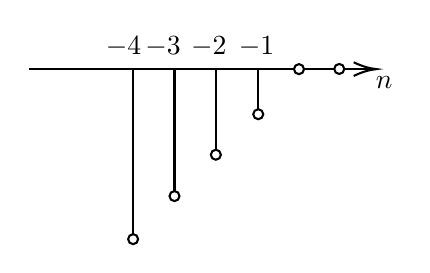
\begin{tikzpicture}[x=0.75pt,y=0.75pt,yscale=-1,xscale=1]
%uncomment if require: \path (0,300); %set diagram left start at 0, and has height of 300

%Straight Lines [id:da8305438567766523] 
\draw    (200.27,190.67) -- (365.77,190.67) ;
\draw [shift={(367.77,190.67)}, rotate = 180] [color={rgb, 255:red, 0; green, 0; blue, 0 }  ][line width=0.75]    (10.93,-3.29) .. controls (6.95,-1.4) and (3.31,-0.3) .. (0,0) .. controls (3.31,0.3) and (6.95,1.4) .. (10.93,3.29)   ;

%Shape: Circle [id:dp5343795865479193] 
\draw  [fill={rgb, 255:red, 255; green, 255; blue, 255 }  ,fill opacity=1 ] (347.47,190.58) .. controls (347.47,189.25) and (348.55,188.17) .. (349.88,188.17) .. controls (351.22,188.17) and (352.3,189.25) .. (352.3,190.58) .. controls (352.3,191.92) and (351.22,193) .. (349.88,193) .. controls (348.55,193) and (347.47,191.92) .. (347.47,190.58) -- cycle ;
%Shape: Circle [id:dp9958561748525927] 
\draw  [fill={rgb, 255:red, 255; green, 255; blue, 255 }  ,fill opacity=1 ] (328.07,190.68) .. controls (328.07,189.35) and (329.15,188.27) .. (330.48,188.27) .. controls (331.82,188.27) and (332.9,189.35) .. (332.9,190.68) .. controls (332.9,192.02) and (331.82,193.1) .. (330.48,193.1) .. controls (329.15,193.1) and (328.07,192.02) .. (328.07,190.68) -- cycle ;
%Straight Lines [id:da3574860753882376] 
\draw    (250.57,272.59) -- (250.57,191.28) ;


%Shape: Circle [id:dp04408180627185376] 
\draw  [fill={rgb, 255:red, 255; green, 255; blue, 255 }  ,fill opacity=1 ] (248.17,272.59) .. controls (248.17,273.92) and (249.24,275) .. (250.57,275) .. controls (251.9,275) and (252.98,273.92) .. (252.98,272.59) .. controls (252.98,271.26) and (251.9,270.18) .. (250.57,270.18) .. controls (249.24,270.18) and (248.17,271.26) .. (248.17,272.59) -- cycle ;
%Straight Lines [id:da7712579502140393] 
\draw    (270.5,251.85) -- (270.5,191.28) ;


%Shape: Circle [id:dp4215879501304003] 
\draw  [fill={rgb, 255:red, 255; green, 255; blue, 255 }  ,fill opacity=1 ] (268.1,251.85) .. controls (268.1,253.18) and (269.17,254.26) .. (270.5,254.26) .. controls (271.83,254.26) and (272.91,253.18) .. (272.91,251.85) .. controls (272.91,250.52) and (271.83,249.44) .. (270.5,249.44) .. controls (269.17,249.44) and (268.1,250.52) .. (268.1,251.85) -- cycle ;
%Straight Lines [id:da39800912811539835] 
\draw    (290.43,231.92) -- (290.43,191.28) ;


%Straight Lines [id:da15358320586768315] 
\draw    (310.86,210) -- (310.86,190.78) ;


%Shape: Circle [id:dp9326128099979845] 
\draw  [fill={rgb, 255:red, 255; green, 255; blue, 255 }  ,fill opacity=1 ] (288.02,231.92) .. controls (288.02,233.25) and (289.1,234.33) .. (290.43,234.33) .. controls (291.76,234.33) and (292.84,233.25) .. (292.84,231.92) .. controls (292.84,230.59) and (291.76,229.51) .. (290.43,229.51) .. controls (289.1,229.51) and (288.02,230.59) .. (288.02,231.92) -- cycle ;
%Shape: Circle [id:dp7866868035269907] 
\draw  [fill={rgb, 255:red, 255; green, 255; blue, 255 }  ,fill opacity=1 ] (308.45,212.41) .. controls (308.45,213.74) and (309.53,214.81) .. (310.86,214.81) .. controls (312.19,214.81) and (313.27,213.74) .. (313.27,212.41) .. controls (313.27,211.08) and (312.19,210) .. (310.86,210) .. controls (309.53,210) and (308.45,211.08) .. (308.45,212.41) -- cycle ;

% Text Node
\draw (224,203) node   {$\dotsc $};
% Text Node
\draw (371.5,197) node   {$n$};
% Text Node
\draw (310,180) node   {$-1$};
% Text Node
\draw (287,180) node   {$-2$};
% Text Node
\draw (265,180) node   {$-3$};
% Text Node
\draw (246,180) node   {$-4$};


\end{tikzpicture}
